\chapter{Grattan survey of students who dropped out}\label{chap:b}

Between 15 December 2017 and 5 January 2018, the Grattan Institute conducted an online survey of students who dropped out of university -- \emph{Incomplete University Survey}. It was hosted on SurveyMonkey and promoted via Grattan's social media channels on Facebook, Twitter and LinkedIn. In addition, the Facebook post was advertised to people in Australia aged between 18 and 50. About 90 per cent of responses came through Facebook. Overall the survey received about 950 responses.

About 100 respondents were excluded either because they did not drop out of university (answered no to question 1) or because they did not answer any subsequent questions.\footnote{Respondents who said no to question 1 were blocked from taking the survey again on the same device.} 
Except for the question on whether the respondent has dropped out (question 1), answers were optional to reduce survey attrition and improve response quality.\footcite[][556--558]{Krosnick1999} 
About 43 respondents dropped out from a sub-bachelor course, 116 from a masters degree, and 55 from a doctorate degree, and are also excluded from our analysis.\footnote{The qualification level of the survey respondents was similar to domestic higher education enrolments.}

For the 646 valid bachelor degree responses, \Cref{fig:25} shows the demographic mix of the online survey respondents compared to commencing students between 2005 and 2016. Two-fifths of respondents grew up in a rural area and nearly a quarter are from the highest socio-economic decile. Both are slightly over-represented in the online survey compared to enrolments.

                % Figure 25
                \begin{figure}
                    \caption{Distribution of Grattan survey respondents and university enrolments\label{fig:25}}%
                    \units{Per cent}
                    \includegraphics[page=38]{atlas/selection_chartdeck.pdf} 
                    \noteswithsource{Bachelor-degree only. IEO is the Index of Education and Occupation.}{Grattan online survey; \textcite{DepartmentofEducationandTraininga}}
                \end{figure}


There are no other comprehensive surveys of Australian students who dropped out to systematically benchmark the online survey results.\footnote{Both the Student Experience Survey and the first-year experience survey ask for reasons from students who consider leaving their institution. But the results are not directly comparable. Nonetheless, the most common reason cited was health or stress related for both surveys, \textcites[][29]{Baik2015}[][74]{SocialResearchCentre/DepartmentofEducationandTraining2017}.} The closest alternative is the Longitudinal Survey of Australian Youth (LSAY). It tracks students aged 15 to 25, meaning that students who dropped out after age 25 are excluded. Grattan's online survey overlaps with the LSAY on one question -- reasons for leaving university.

Restricting the online survey to those aged 25 or younger and who left their bachelor degree after 2007, \Cref{fig:26} compares results from the two surveys.\footnote{The LSAY 2006 cohort is used because it is the most recent complete survey.} 
Respondents can choose multiple reasons, but many in the Grattan survey chose only one. In each survey, a similar proportion of respondents chose health and financial reasons. But LSAY respondents were much more likely to also pick other reasons, which could partly be explained by a greater tendency of LSAY respondents to choose multiple reasons. The average number of items selected in the Grattan survey was 2.4; for LSAY it was 3.2.\footnote{The reasons for these substantial differences are unclear. One reason could be that our online survey had a number of single-response questions preceding the reason-for-leaving question.}

LSAY subsequently asks for the main reason for dropping out. Using this question, which allows for only one reason per respondent, the results of the two surveys are more comparable. But there are still substantial discrepancies, as \Cref{fig:26} shows (orange bar and black line).

                % Figure 26
                \begin{figure*}
                    \caption{Comparing LSAY and the Grattan online survey results\label{fig:26}}%
                    \units{Per cent}
                    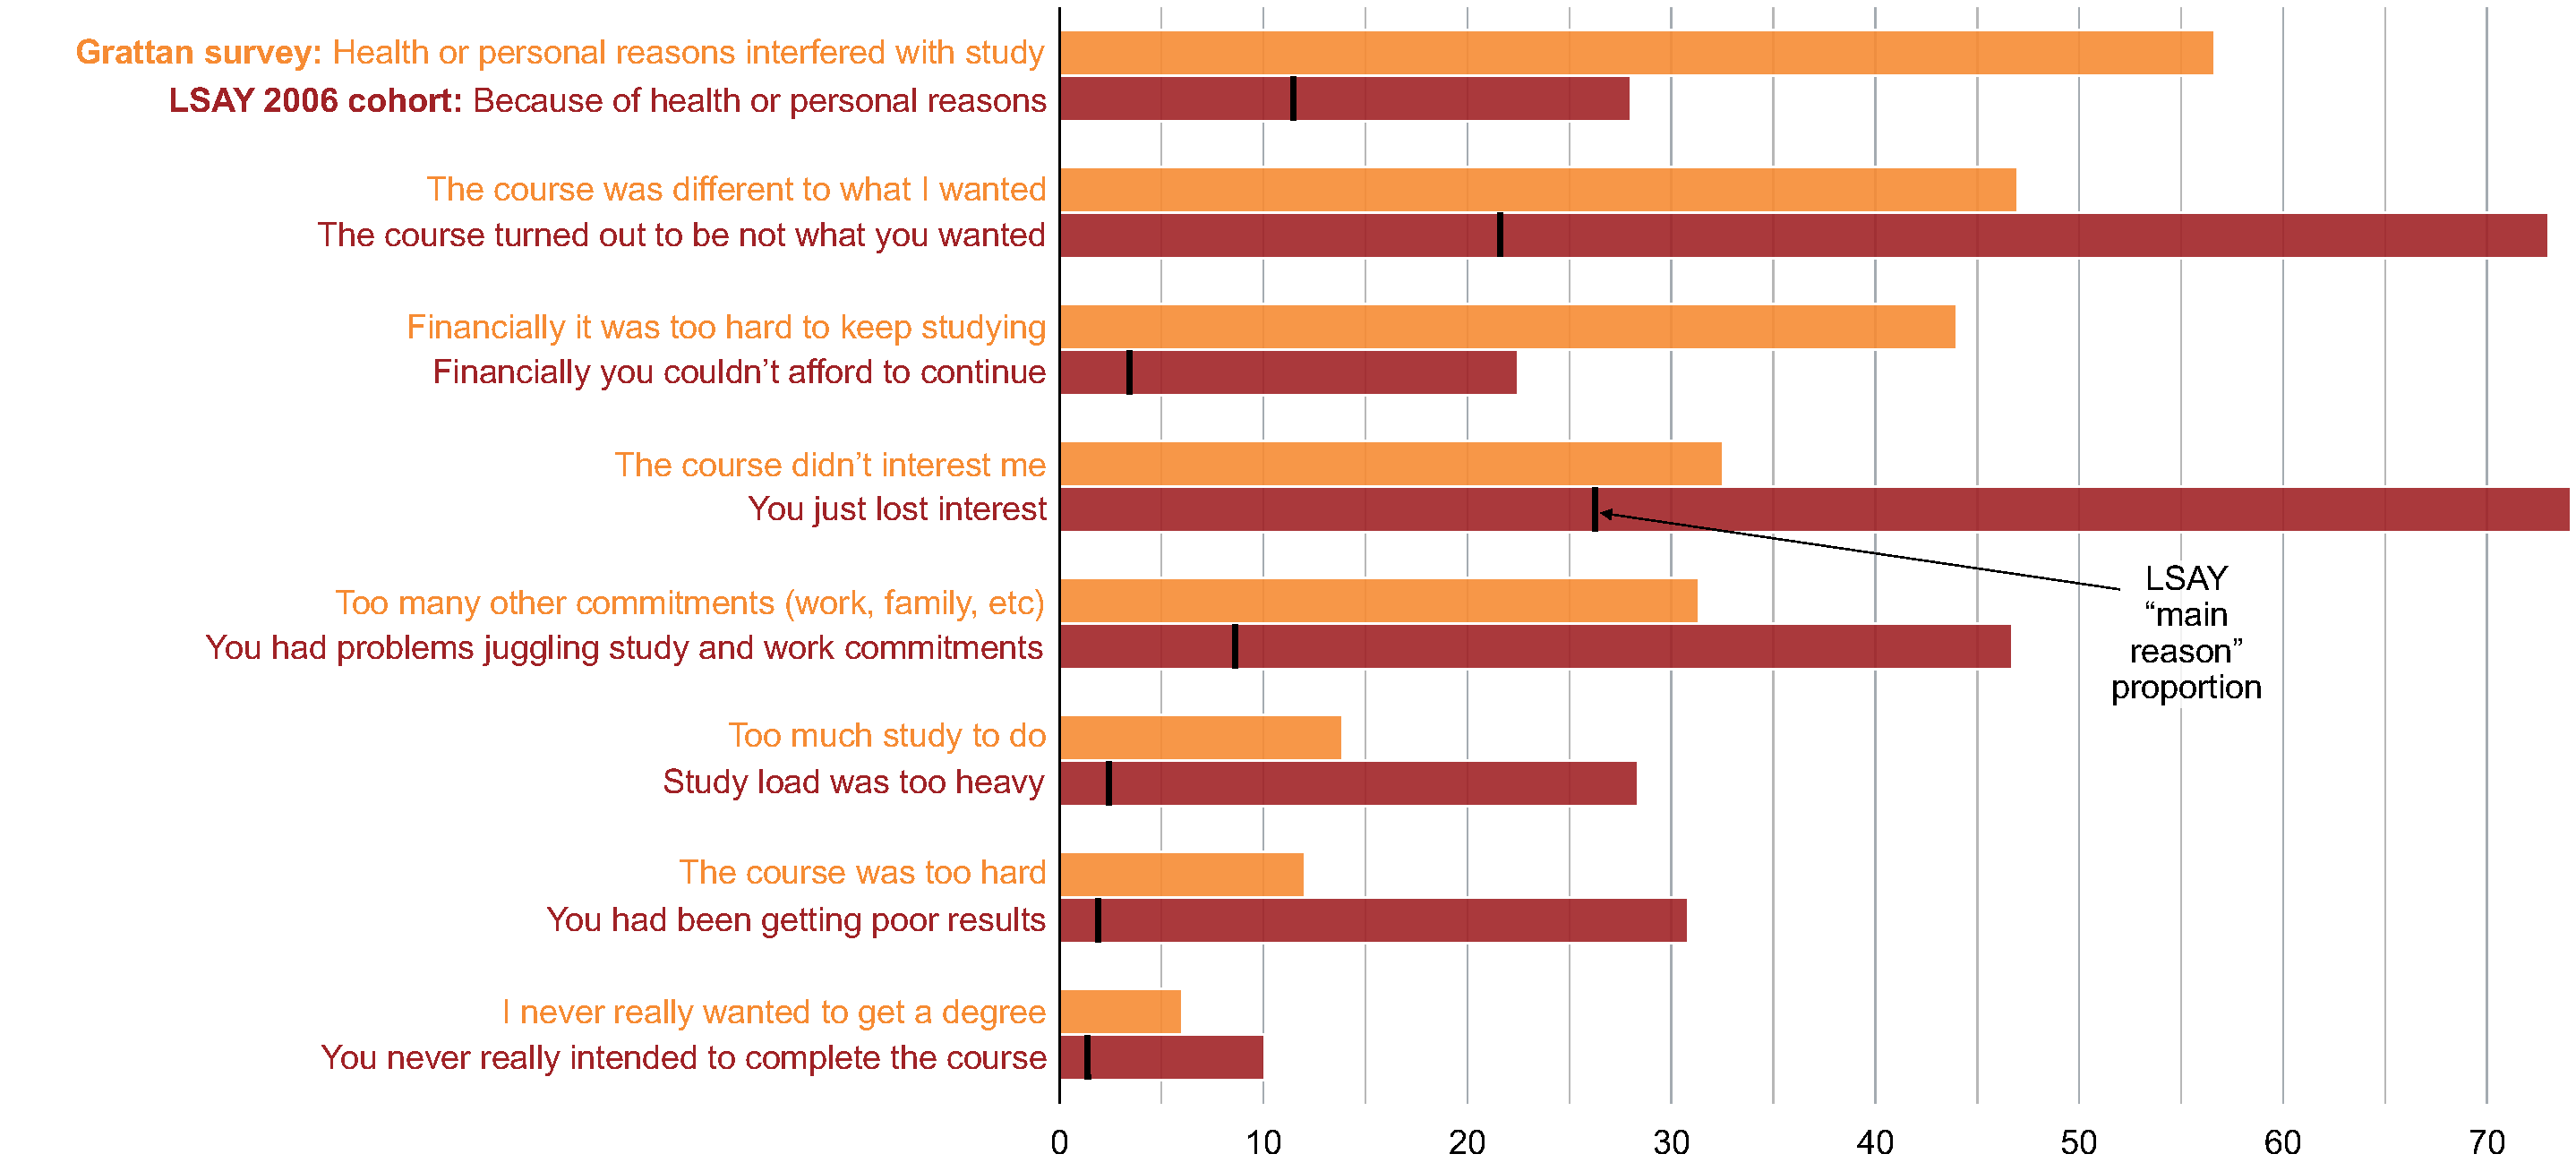
\includegraphics[page=1, width=2.15\columnwidth]{atlas/reasons_leaving_fullpage.pdf} 
                    \noteswithsource{Using LSAY 2006 cohort, there are 289 students who dropped out by the age of 25. To make the Grattan online survey more consistent with LSAY (for this chart only), respondents aged above 25 and those who dropped out were excluded, resulting in 166 observations. Respondents can choose multiple reasons (not for the main reason question). Five additional options that are available in LSAY but omitted from the Grattan survey are: ``just wanted to get a job, apprenticeship or traineeship'' (11 per cent), ``never really wanted to study'' (2 per cent), ``it wouldn't have led to a good job or career'' (3 per cent), ``because problems with access or transport'' (less than 1 per cent), and ``other'' (6 per cent).}
                    {\textcites[][]{NCVER2014}; Grattan online survey}
                \end{figure*}




% /////TABLE
%%START LONGTABLE
    \onecolumn
    \bgroup
    \def\arraystretch{1.1}
    \begin{longtable}{p{.7cm}p{18.6cm}p{2cm}p{2cm}}
    
    \caption{Incomplete University Survey Questions}\label{tbl:surveyquestions} \\
    
    \toprule & \textbf{Question}  &   \textbf{Type}   &   \textbf{Response Rate} \\ 
    \hline 
    \endfirsthead
    
    \multicolumn{4}{l}
    {\footnotesize{{\textbf{\tablename\ \thetable{}} -- \textit{continued from previous page}}}} \\
    \toprule
    & \textbf{Question}  &   \textbf{Type}   &   \textbf{Response Rate} \\ 
    \hline 
    \endhead
    
    
    
    \multicolumn{4}{r}{\footnotesize\emph{Continued on next page}} \\
    \endfoot
    
    \hline
    \endlastfoot
    
        Q1    & Have you ever dropped out of a university degree in Australia? \newline \textit{[Options: yes; no]}      & Required, select Y/N          & 100.0\% \\
        \midrule
        Q2    & What level was the incomplete degree? \newline \textit{[Options: diploma/associates degree; masters degree (research); masters degree (coursework); bachelor degree; doctorate degree]} & Select one & 99.4\% \\
        \midrule
        Q3    & What field was the incomplete degree in? \newline \textit{[Options: agriculture; architecture, commerce; creative arts; education; engineering; hospitality; humanities; information technology; law; medical; nursing; other health; science; other (please specify)]} & Select one + other & 100.0\% \\
        \midrule
        Q4    & What year did you start? & Text  & 99.4\% \\
        \midrule
        Q5    & What year did you leave your incomplete degree? & Text  & 99.3\% \\
        \midrule
        Q6    & What was your highest level of education before starting the degree? \newline \textit{[Options: had not finished year 12; finished year 12; cert I/II; cert III/IV; diploma/associate degree; bachelor degree; postgraduate; other (please specify)]} & Select one & 99.5\% \\
        \midrule
        Q7    & What is your highest level of education now? \newline \textit{[Options from Q6]} & Select one & 99.8\% \\
        \midrule
        Q8    & Do you know how much HELP debt you owe? \newline \textit{[Options: yes; no]} & Select one, logic to Q9 & 99.5\% \\
        \midrule
        Q9    & How much HELP debt do you owe? (Optional) & Text  & 53.4\% \\
        \midrule
        Q10   & Were there any benefits from the time you spent doing the incomplete degree? \newline \textit{[Options: it helped clarify my careers goals; it taught me useful skills; it was interesting; I made lasting friendships/connections; attending university helped me get employed; no benefits]} & Select many & 92.2\% \\
        \midrule
        Q11   & Please provide more details & Text  & 71.5\% \\
        \midrule
        Q12   & Below is a list of reasons why people might leave their course. Check any that were a factor in your own decision. \newline \textit{[Options: health or personal reasons interfered with study; financially it was too hard to keep studying; the course was different to what I wanted; too much study to do; the course was too hard; too many other commitments (work, family, \etc{}); the course didn't interest me; I never really wanted to get a degree]} & Select many & 79.0\% \\
        \midrule
        Q13   & Please provide more details & Text  & 79.3\% \\
        \midrule
        Q14   & In leaving your degree, did you ever feel that you let anyone down? \newline \textit{[Options: yes; maybe; no]} & Select one & 94.2\% \\
        \midrule
        Q15   & If yes, can you elaborate? & Text  & 65.0\% \\
        \midrule
        Q16   & Knowing what you know now, would you still have made the decision to start your degree? \newline \textit{[Options: yes; no; unsure]} & Select one & 91.7\% \\
        \midrule
        Q17   & Can you go into more detail? & Text  & 78.7\% \\
        \midrule
        Q18   & Also knowing what you know now, would you still have decided to leave your degree? \newline \textit{[Options: yes; no; unsure]} & Select one & 91.5\% \\
        \midrule
        Q19   & Can you go into more detail? & Text  & 73.8\% \\
        \midrule
        Q20   & Do you think you would be in a better position now if you had finished your degree? \newline \textit{[Instruction on scale: 1= much worse; 4= about the same; 7= much better]} & Scale 1-7 & 78.4\% \\
        \midrule
        Q21   & Before starting your degree, what kind of information would have benefited you? & Text  & 78.0\% \\
        \midrule
        Q22   & Would you still have started your degree if you had more information before applying? \newline \textit{[Options: yes; no; unsure]} & Select one & 91.9\% \\
        \midrule
        Q23   & Do you think you will enrol in university again in the future? \newline \textit{[Options: yes; no; unsure]} & Select one & 92.3\% \\
        \midrule
        Q24   & Any further comments? & Text  & 47.1\% \\
        \midrule
        Q25   & Would you like to answer some optional demographic questions? \newline \textit{[Options: yes; \textbf{no, finish the survey}]} & Select one & 92.1\% \\
        \midrule
        Q26   & What is your age? & Text  & 84.5\% \\
        \midrule
        Q27   & In which country were you born? & Select one & 84.2\% \\
        \midrule
        Q28   & Did you grow up in a city or rural location? \newline \textit{[Options: city; rural]} & Select one & 84.1\% \\
        \midrule
        Q29   & What was your postcode growing up? & Text  & 78.0\% \\
        \midrule
        Q30   & What institution did you attempt your degree? & Text  & 82.6\% \\
        \bottomrule
        
    \end{longtable}
    \egroup
    \twocolumn